\begin{frame}
\begin{alertblock}{Передімною було поставлено завдання:}
	\begin{itemize}
		\item 1. Побудувати алгоритм для чотирикрокового методу мінімізації функцій;
		\item 2. Перевірити його доцільність на тестових функціях;
		\item 3. Порівняти 3-х і 4-х крокові методи мінімізації функцій.
	\end{itemize}
\end{alertblock}
\begin{alertblock}{Що я зробила:}
	Я побудувала алгоритм для чотирикрокового методу мінімізації функцій та обґрунтувала його належність до методів спряжених напрямків. Далі я перевірила алгоритм на тестових функціях і порівняла його з трикроковим методом мінімізації функцій. 
\end{alertblock}
\end{frame}

\begin{frame}
\frametitle{Вступ} 
На сучасному етапі розвитку науки та комп'ютерних технологій теорія чисельних методів нелінійного програмування є досить розвиненою. Проте ще досить важко дати чіткі рекомендації щодо застосування того чи іншого методу.

У літературі описані багатокрокові методи, а саме - двокроковий метод спряжених градієнтів. Цей метод вважається досить ефективним для задач великої розмірності. Метод спряжених градієнтів має перевагу перед однокроковими градієнтрими методами, бо він у більшій мірі враховує геометричні властивості цільової функції. Опираючись на цю інформацію, можна піти далі і розглянути трикрокові, чотирикрокові, п'ятикрокові і т.д. методи.

У роботі розглянуто чотирикроковий метод, дано чисельну порівняльну характеристику у порівнянні з трикроковим методом.
\end{frame}

\begin{frame}[shrink=5]
\frametitle{Алгоритм чотирикрокового методу} 
Розглянемо задачу мінімізації функції багатьох змінних без обмежень
$$ \phi (x) \to min, \; x \in \mathbb{R}^n , \eqno(1) $$ де  
$$ \phi (x) : \mathbb{R}^n \to \mathbb{R}^1 \text{ - неперервно диференційовна функція } $$
Позначимо її градієнт через $  \phi'(x) $.
А для її розв'язання розглянемо чотирикроковий метод з таким алгоритмом:
$$ x^{k + 1} = x^k + \beta_k s^k, \; k = 0, 1,\ldots $$
$$
S = \quad
\begin{cases}
-\phi' (x^k) & , k = 0 \\
-\phi' (x^k) + \gamma_1^{k-1}s^{k-1} & , k = 1 \\
-\phi' (x^k) + \gamma_1^{k-1}s^{k-1} + \gamma_2^{k-2}s^{k-2} & , k = 2 \\
-\phi' (x^k) + \gamma_1^{k-1}s^{k-1} + \gamma_2^{k-2}s^{k-2} +  \gamma_3^{k-3}s^{k-3} & , k = 3, \ldots
\end{cases}	\eqno(2)
$$
де $ \;\;\;\;\;\;\;\, x^0, x^1, \dotsc , x^k, \dotsc $ - послідовні наближення \\
$s^0, s^1, \dotsc , s^k, \dotsc $ - напрямки спуску \\
$\beta_k, \gamma_j^m (j = \overline{1,3}) $ - числові параметри 

Параметр $\beta_k$ будемо визначати з умови:
$$ \beta_k : \min_{\beta\geq0} \phi(x^k + \beta s^k) \eqno(3)$$
\end{frame}

\begin{frame}[shrink=0]
\frametitle{Теоретичні положення методу} 
Розглянемо деякі властивості методу при умові, що функція $\phi(x)$ є квадратичною.
$$  \phi(x) = \frac{1}{2} (Ax,x) + (b,x) + c \eqno(4) $$
Побудуємо систему взаємно спряжених напрямків за правилом (2). 
$$ 0 = (s^k, As^{k-1}) = -(\phi'(x^k), As^{k-1}) + \gamma_1^{k-1}(s^{k-1}, As^{k-1}) + $$
$$ + \gamma_2^{k-2}\underbrace{(s^{k-2}, As^{k-1})}_{0} + \gamma_3^{k-3}\underbrace{(s^{k-3}, As^{k-1})}_{0}  \Longrightarrow$$ 
$$\gamma_1^{k-1} = \dfrac{(\phi'(x^k), As^{k-1})}{(s^{k-1}, As^{k-1})} \eqno(5)$$
Аналогічно отримаємо: 
$$\gamma_2^{k-2} = \dfrac{(\phi'(x^k), As^{k-2})}{(s^{k-2}, As^{k-2})} \eqno(6)$$
$$\gamma_3^{k-3} = \dfrac{(\phi'(x^k), As^{k-3})}{(s^{k-3}, As^{k-3})} \eqno(7)$$
\end{frame}

\begin{frame}
\begin{alertblock}{Теорема 1.}
	\textit{Для диференційовної функції $\phi(x)$ послідовність $\{x^k\}$, що побудована за (2), (5), (6), (7), така, що $ (\phi'(x^{k+1}), s^k) = 0, \, k = 0, 1, \ldots $} 
\end{alertblock}
\begin{alertblock}{Теорема 2.}
	\textit{Вектори $\phi'(x^k) \; \text{i} \; \phi'(x^{k+1}) $ ортогональні, $ k = 0, 1, \ldots $} 
\end{alertblock}
\begin{alertblock}{Теорема 3.}
	\textit{Нехай $x^0 \in \mathbb{R}^n , \text{ точки } x^1, x^2, \ldots , x^{n-1}$  і вектори $s^0, s^1, \ldots, s^{n-1} $ отримані за формулами  (2), (5), (6), (7) і 
		$ \phi'(x^k) \neq 0 $ \\ $ (k = \overline{0,n-1}) $, тоді вектори $ s^0, s^1, \ldots, s^{n-1} $ взаємно спряжені, а градієнти $ \phi'(x^0), \phi'(x^1), \ldots,  \phi'(x^{n-1}) $ взаємно ортогональні.} 
\end{alertblock}
Отже розглянутий чотирьохкроковий метод (2), (5), (6), (7) належить до методів спряжених напрямків.
\end{frame}

\begin{frame}
Тепер сформулюємо чотирикроковий метод для мінімізації неквадратичних функцій. \\
Для цього перетворимо формули  (5), (6), (7) так, щоб до них не входила матриця $A$.
$$ \gamma_1^{k-1} = \dfrac{(\phi'(x^k), As^{k-1})}{(s^{k-1}, As^{k-1})} = \dfrac{(\phi'(x^k), \phi'(x^k) - \phi'(x^{k-1}))}{\lVert \phi'(x^{k-1}) \rVert^2}  \eqno(8)$$
$$ \gamma_2^{k-2} = \dfrac{(\phi'(x^k), As^{k-2})}{(s^{k-2}, As^{k-2})} =  \dfrac{(\phi'(x^k), \phi'(x^{k-1}) - \phi'(x^{k-2}))}{\lVert \phi'(x^{k-2}) \rVert^2} \eqno(9) $$
$$ \gamma_3^{k-3} = \dfrac{(\phi'(x^k), As^{k-3})}{(s^{k-3}, As^{k-3})} =  \dfrac{(\phi'(x^k), \phi'(x^{k-2}) - \phi'(x^{k-3}))}{\lVert \phi'(x^{k-3}) \rVert^2} \eqno(10) $$

Отже, для неквадратичних функцій, чотирикроковий метод має вигляд (2), (8), (9), (10)
\end{frame}

\begin{frame}
\frametitle{Обчислювальний експеримент} 
Зробимо аналіз роботи описаного чотирикрокового методу порівнянно із трикроковим методом. Для порівняння використаємо такі показники, як точність отриманного розв'язку та кількість проведених ітерацій. Під кількістю ітерацій будемо розуміти кількість отриманих послідовних наближень до розв'язку задачі. Зауважимо, що кількість обчислень значень функції та її градієнту у чотирикроковому методі не змінюється порівняно із трикроковим.

Для розрахунків використовувалася мова програмування Python. Обчислення проводилися із точністю $\varepsilon = 10^{-6}, 10^{-8}$. Критерій зупинки процесу обчислень полягав у одночасному виконанні трьох умов:
$$
\phi(x^{k-1}) - \phi(x^{k}) < \varepsilon(1 + |\phi(x^{k})|), $$
$$\lVert x^{k-1} - x^{k} \rVert < \sqrt{\varepsilon}(1 + \lVert x^{k} \rVert), $$
$$ \lVert \phi'(x^{k})\rVert \leq \sqrt[3]{\varepsilon}(1 + |\phi(x^{k})|) 
$$
Пунктирною лінією позначений процес мінімізіції трикроковим методом, суцільною - чотирикроковим.
\end{frame}

\begin{frame}
\frametitle{Задача 1. $\phi(x) = \left(- x_{1} + 1\right)^{2} + 100 \left(- x_{1}^{2} + x_{2}\right)^{2}$} 
Точний розв'язок задачі: x* = [1, 1] f* = 0
	{\scriptsize  \begin{center}
		\begin{tabular}{|c|c|c|c|c|c|p{0.1\linewidth}|}
			\hline
			$\varepsilon$ & $x_0$ & $f(x_0)$ & Метод мінімізації & $x^* \text{ - отриманий розв'язок} $  & $f(x^*)$ & Кількість ітерацій \\
			\hline
			\multirow{8}{*}{$10^{-6}$} & \multirow{2}{*}{[-1.2, 1]} & \multirow{2}{*}{24.2} & 4 кроковий & [ 1.00027  1.00053] & 0 & 93 \\
			\hhline{~~~----} & & & 3 кроковий & [ 1.00069  1.00137] & 0.0 & 29 \\
			\hhline{~------}	
			& \multirow{2}{*}{[1, -1.2]} & \multirow{2}{*}{484} & 4 кроковий & [ 0.99995  0.99991] & 0 & 81 \\
			\hhline{~~~----} & & & 3 кроковий & [ 0.99994  0.99988] & 0 & 21 \\
			\hhline{~------}
			& \multirow{2}{*}{[0, 0]} & \multirow{2}{*}{1} & 4 кроковий & [ 1.00015  1.00029] & 0 & 42 \\
			\hhline{~~~----} & & & 3 кроковий & [ 1.00014  1.00029] & 0 & 24 \\
			\hhline{~------}	
			& \multirow{2}{*}{[-1, -1]} & \multirow{2}{*}{404} & 4 кроковий & [ 0.99998  0.99995] & 0 & 59 \\
			\hhline{~~~----} & & & 3 кроковий & [ 0.99992  0.99985] & 0 & 25 \\
			\hline	
		\end{tabular}
	\end{center}}
\end{frame}

\begin{frame}
\begin{columns}
	\begin{column}[t]{0.5\linewidth}
		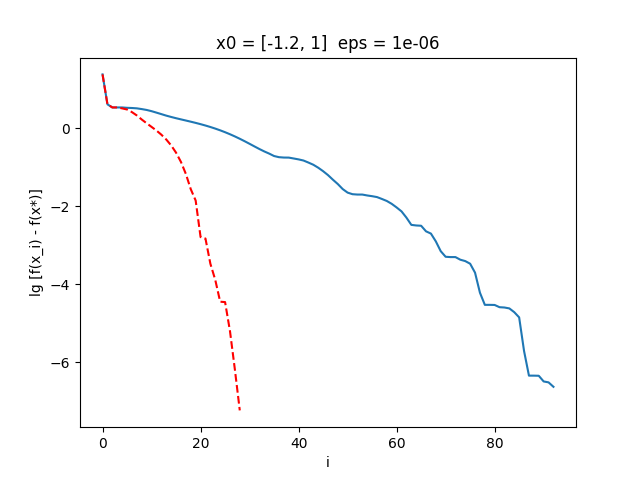
\includegraphics[width=0.9\linewidth]{Figure_1} \\
		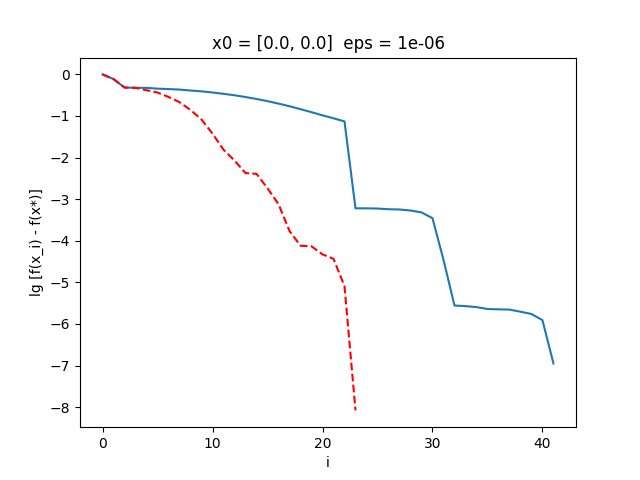
\includegraphics[width=0.9\linewidth]{Figure_1_2}
	\end{column}
	
	\begin{column}[t]{0.5\linewidth}
		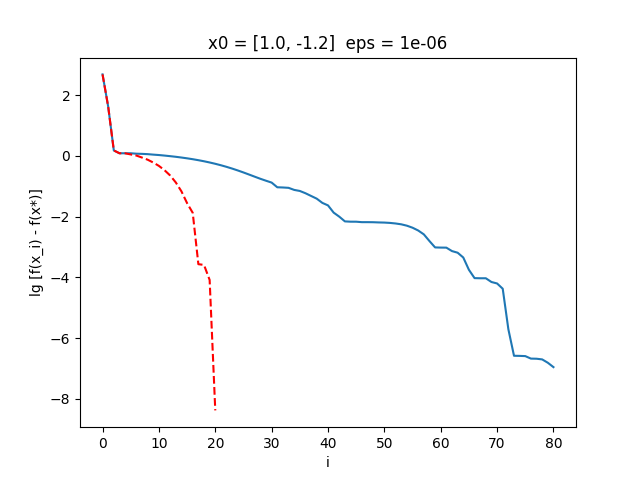
\includegraphics[width=0.9\linewidth]{Figure_1_1} \\
		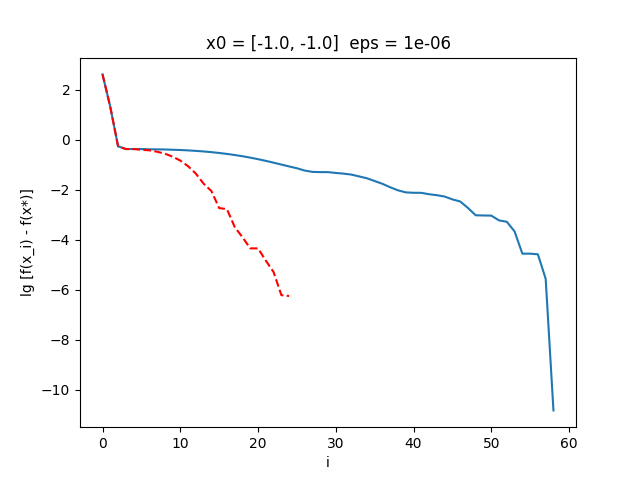
\includegraphics[width=0.9\linewidth]{Figure_1_3}
	\end{column}
\end{columns}
\end{frame}

\begin{frame}
\frametitle{Задача 1. $\phi(x) = \left(- x_{1} + 1\right)^{2} + 100 \left(- x_{1}^{2} + x_{2}\right)^{2}$} 
Точний розв'язок задачі: x* = [1, 1] f* = 0
{\scriptsize  \begin{center}
		\begin{tabular}{|c|c|c|c|c|c|p{0.1\linewidth}|}
			\hline
			$\varepsilon$ & $x_0$ & $f(x_0)$ & Метод мінімізації & $x^* \text{ - отриманий розв'язок} $  & $f(x^*)$ & Кількість ітерацій \\
			\hline
			\multirow{8}{*}{$10^{-8}$}	& \multirow{2}{*}{[-1.2, 1]} & \multirow{2}{*}{24.2} & 4 кроковий & [ 0.99999  0.99999] & 0 & 98 \\
			\hhline{~~~----} & & & 3 кроковий & [ 0.99997  0.99994] & 0 & 35 \\
			\hhline{~------}
			& \multirow{2}{*}{[1, -1.2]} & \multirow{2}{*}{484} & 4 кроковий & [ 1.       0.99999] & 0 & 32 \\
			\hhline{~~~----} & & & 3 кроковий & [ 1.  1.] & 0 & 25 \\
			\hhline{~------}
			& \multirow{2}{*}{[0, 0]} & \multirow{2}{*}{1} & 4 кроковий & [ 0.99993  0.99985] & 0 & 24 \\
			\hhline{~~~----} & & & 3 кроковий & [ 1.  1.] & 0 & 19 \\
			\hhline{~------}
			& \multirow{2}{*}{[-1, -1]} & \multirow{2}{*}{404} & 4 кроковий & [ 0.99998  0.99996] & 0 & 20 \\
			\hhline{~~~----} & & & 3 кроковий & [ 1.  1.] & 0 & 16 \\
			\hline	
		\end{tabular}
\end{center}}
\end{frame}

\begin{frame}
\begin{columns}
	\begin{column}[t]{0.5\linewidth}
		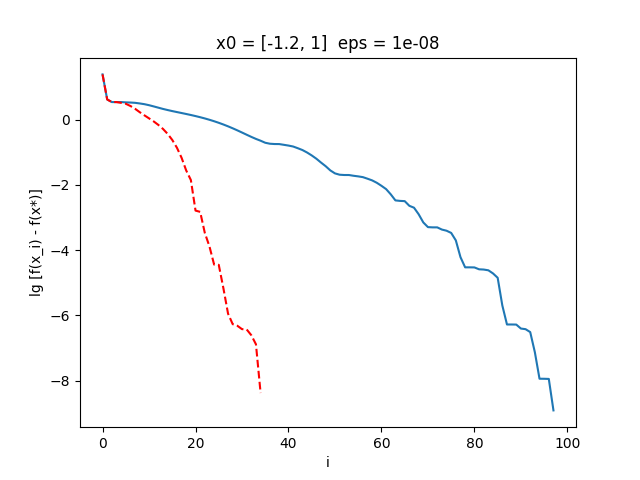
\includegraphics[width=0.9\linewidth]{Figure_1_1_1} \\
		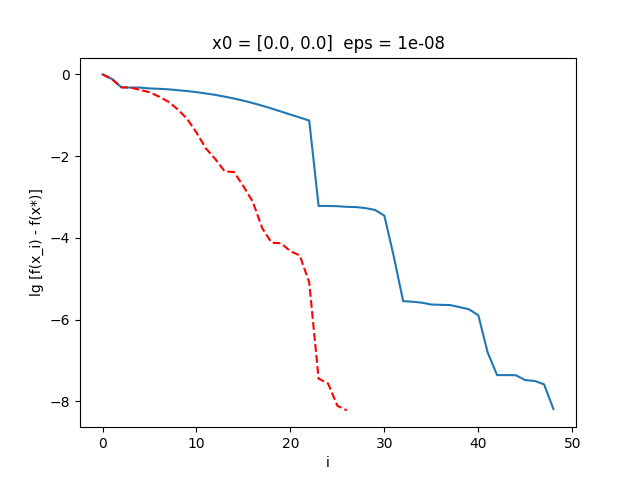
\includegraphics[width=0.9\linewidth]{Figure_1_1_3}
	\end{column}
	
	\begin{column}[t]{0.5\linewidth}
		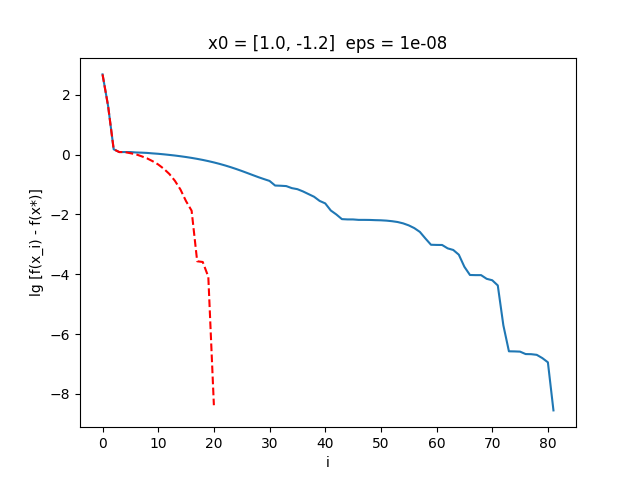
\includegraphics[width=0.9\linewidth]{Figure_1_1_2} \\
		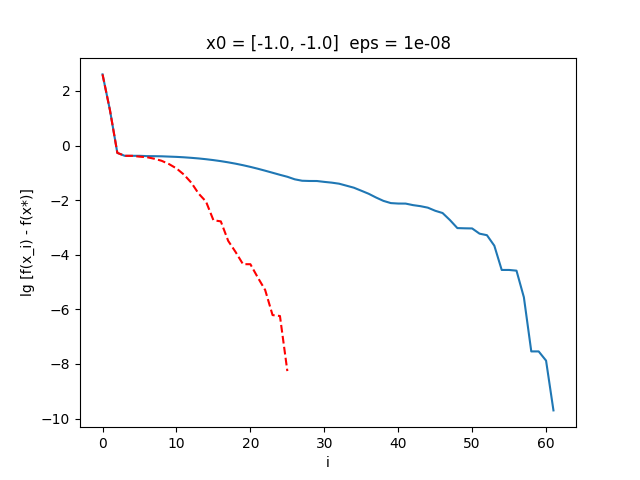
\includegraphics[width=0.9\linewidth]{Figure_1_1_4}
	\end{column}
\end{columns}
\end{frame}

\begin{frame}
\frametitle{Задача 2. $\phi(x) = \left(x_{1} + 10 x_{2}\right)^{2} + 10 \left(x_{1} - x_{4}\right)^{4} + \left(x_{2} - 2 x_{3}\right)^{4} + 5 \left(x_{3} - x_{4}\right)^{2}$} 
Точний розв'язок задачі: x* = [0, 0, 0, 0] f* = 0
{\scriptsize  \begin{center}
		\begin{tabular}{|c|c|c|p{0.11\linewidth}|c|c|p{0.07\linewidth}|}
			\hline
			$\varepsilon$ & $x_0$ & $f(x_0)$ & Метод мінімізації & $x^* \text{ - отриманий розв'язок} $  & $f(x^*)$ & Кількість ітерацій \\
			\hline
			\multirow{8}{*}{$10^{-6}$} & \multirow{2}{*}{[3, -1, 0, 1]} & \multirow{2}{*}{215} & 4 кроковий & [ 0.05 -0.005  0.03  0.03] & 3e-05 & 36 \\
			\hhline{~~~----} & & & 3 кроковий & [ 0.0008  -0.00008 -0.008 -0.003] & 0.0 & 36 \\
			\hhline{~------}
			& \multirow{2}{*}{[1, 1, 1, 1]} & \multirow{2}{*}{122} & 4 кроковий & [-0.069  0.0069 -0.04 -0.0411] & 7e-05 & 43 \\
			\hhline{~~~----} & & & 3 кроковий & [-0.048  0.004 -0.025 -0.025] & 1e-05 & 21 \\
			\hhline{~------}
			& \multirow{2}{*}{[-1, 1, -1, 1]} & \multirow{2}{*}{342} & 4 кроковий & [-0.086  0.008 -0.048 -0.048] & 0.00014 & 38 \\
			\hhline{~~~----} & & & 3 кроковий & [ 0 -0 -0.02 -0.01] & 0.0 & 29 \\
			\hhline{~------}
			& \multirow{2}{*}{[0, 2, -1, 1]} & \multirow{2}{*}{686} & 4 кроковий & [ 0.002 -0.0002 0.0015  0.0015] & 0.0 & 44 \\
			\hhline{~~~----} & & & 3 кроковий & [-0.03  0.004 -0.0096 -0.0096] & 1e-05 & 27 \\
			\hline	
		\end{tabular}
\end{center}}
\end{frame}

\begin{frame}
\begin{columns}
	\begin{column}[t]{0.5\linewidth}
		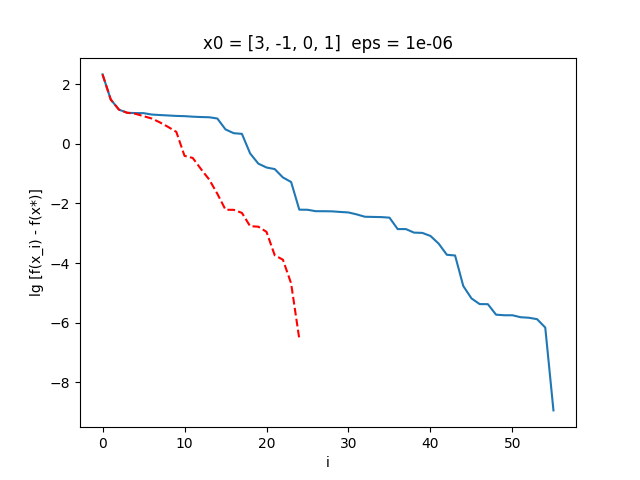
\includegraphics[width=0.9\linewidth]{Figure_2_1} \\
		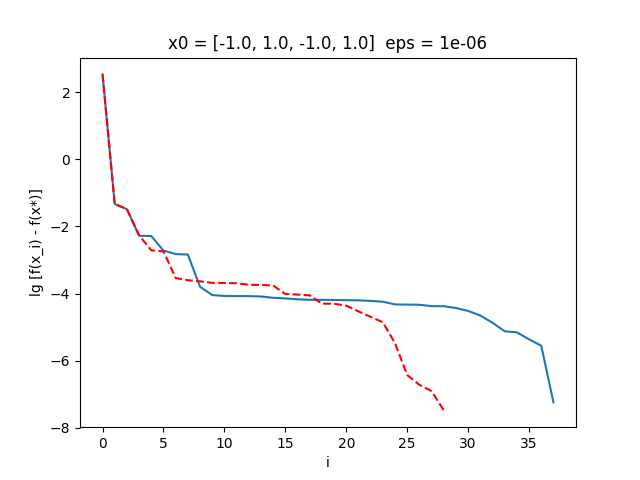
\includegraphics[width=0.9\linewidth]{Figure_2_3}
	\end{column}
	
	\begin{column}[t]{0.5\linewidth}
		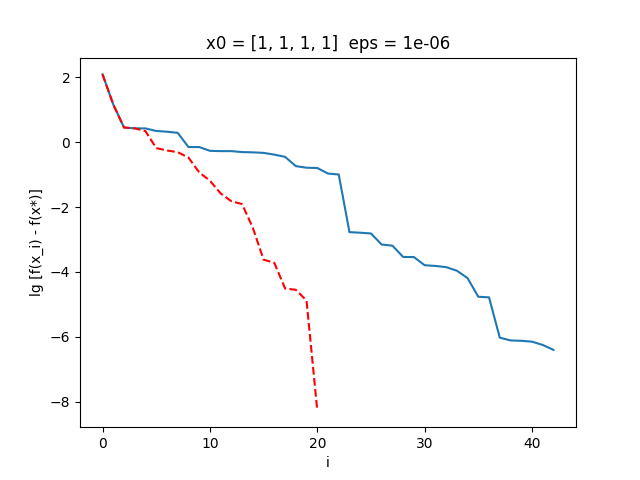
\includegraphics[width=0.9\linewidth]{Figure_2_2} \\
		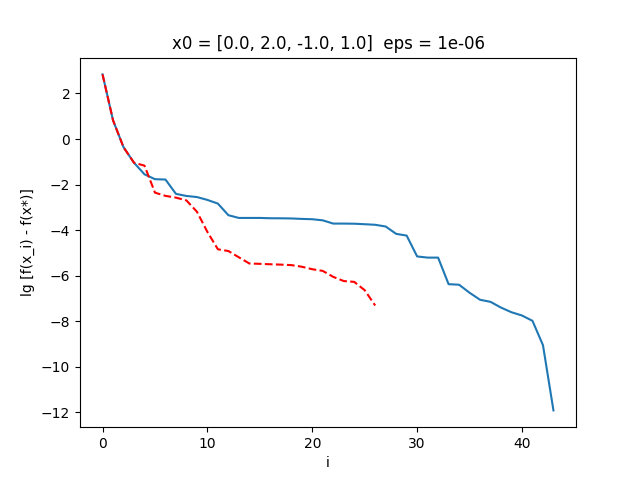
\includegraphics[width=0.9\linewidth]{Figure_2_4}
	\end{column}
\end{columns}
\end{frame}

\begin{frame}
\frametitle{Задача 2. $\phi(x) = \left(x_{1} + 10 x_{2}\right)^{2} + 10 \left(x_{1} - x_{4}\right)^{4} + \left(x_{2} - 2 x_{3}\right)^{4} + 5 \left(x_{3} - x_{4}\right)^{2}$} 
Точний розв'язок задачі: x* = [0, 0, 0, 0] f* = 0
{\scriptsize  \begin{center}
		\begin{tabular}{|p{0.03\linewidth}|c|p{0.03\linewidth}|p{0.11\linewidth}|c|c|p{0.07\linewidth}|}
			\hline
			$\varepsilon$ & $x_0$ & $f(x_0)$ & Метод мінімізації & $x^* \text{ - отриманий розв'язок} $  & $f(x^*)$ & Кількість ітерацій \\
			\hline
			\multirow{8}{*}{$10^{-8}$} & \multirow{2}{*}{[3, -1, 0, 1]} & \multirow{2}{*}{215} & 4 кроковий & [-0.02558  0.00256 -0.01165 -0.01175] & 0 & 56 \\
			\hhline{~~~----} & & & 3 кроковий & [ 0.00019 -0.00002 -0.00241 -0.00241] & 0 & 34 \\
			\hhline{~------}
			& \multirow{2}{*}{[1, 1, 1, 1]} & \multirow{2}{*}{122} & 4 кроковий & [ 0.00081 -0.00008 -0.00795 -0.00794] & 0 & 106 \\
			\hhline{~~~----} & & & 3 кроковий & [-0.02441  0.00244 -0.01503 -0.01505] & 0 & 37 \\
			\hhline{~------}
			& \multirow{2}{*}{[-1, 1, -1, 1]} & \multirow{2}{*}{342} & 4 кроковий & [ 0.00905 -0.0009  -0.00682 -0.00667] & 0 & 83 \\
			\hhline{~~~----} & & & 3 кроковий & [-0.00833  0.00083 -0.00384 -0.00385] & 0 & 44 \\
			\hhline{~------}
			& \multirow{2}{*}{[0, 2, -1, 1]} & \multirow{2}{*}{686} & 4 кроковий & [ 0.00071 -0.00007  0.00963  0.00962] & 0 & 40 \\
			\hhline{~~~----} & & & 3 кроковий & [ 0.00041 -0.00004 -0.00281 -0.00281] & 0 & 62 \\
			\hline
		\end{tabular}
\end{center}}
\end{frame}

\begin{frame}
\begin{columns}
	\begin{column}[t]{0.5\linewidth}
		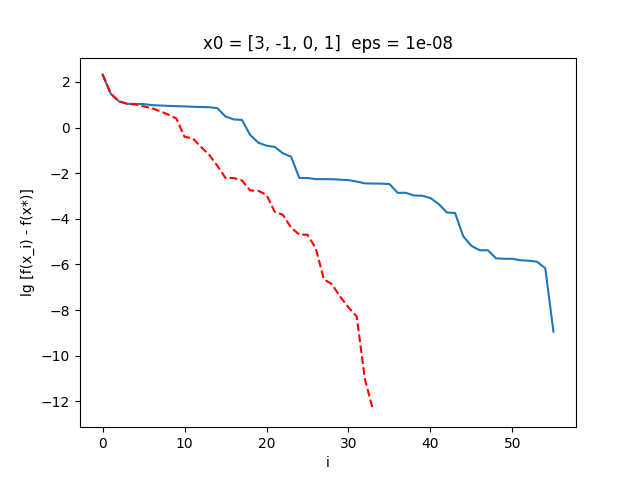
\includegraphics[width=0.9\linewidth]{Figure_2_1_3} \\
		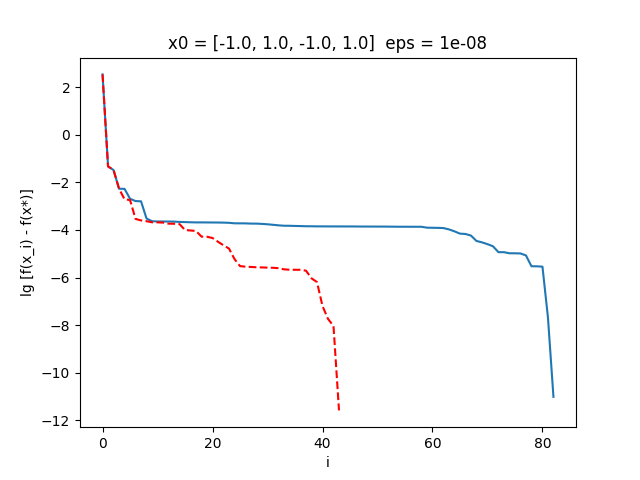
\includegraphics[width=0.9\linewidth]{Figure_2_1_2}
	\end{column}
	
	\begin{column}[t]{0.5\linewidth}
		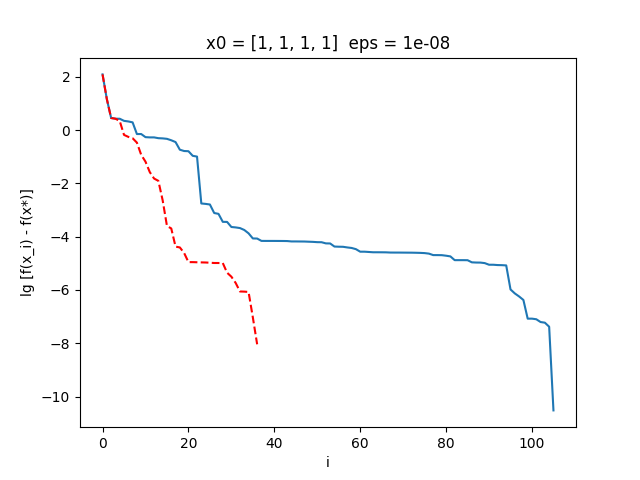
\includegraphics[width=0.9\linewidth]{Figure_2_1_4} \\
		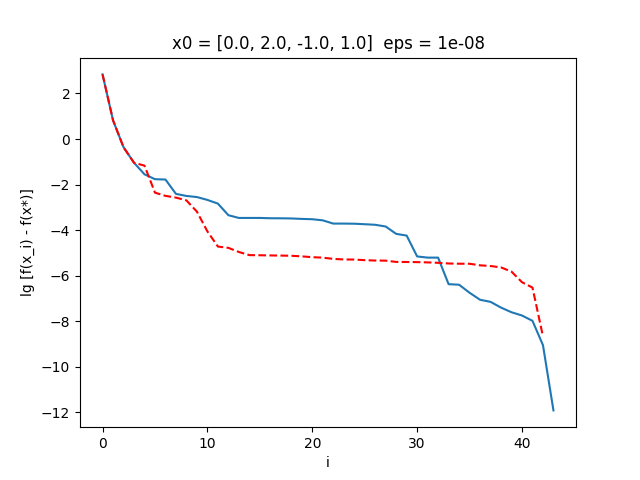
\includegraphics[width=0.9\linewidth]{Figure_2_1_1}
	\end{column}
\end{columns}
\end{frame}

\begin{frame}
\frametitle{Задача 3. $\phi(x) = \left(- x_{1} \left(- x_{2} + 1\right) + 1.5\right)^{2} + \left(- x_{1} \left(- x_{2}^{2} + 1\right) + 2.25\right)^{2} + \left(- x_{1} \left(- x_{2}^{3} + 1\right) + 2.625\right)^{2}$} 
Точний розв'язок задачі: x* = [3, 0.5] f* = 0
{\scriptsize  \begin{center}
		\begin{tabular}{|p{0.03\linewidth}|c|p{0.03\linewidth}|p{0.11\linewidth}|c|c|p{0.08\linewidth}|}
			\hline
			$\varepsilon$ & $x_0$ & $f(x_0)$ & Метод мінімізації & $x^* \text{ - отриманий розв'язок} $  & $f(x^*)$ & Кількість ітерацій \\
			\hline
			\multirow{8}{*}{$10^{-6}$} & \multirow{2}{*}{[2, 0.2]} & \multirow{2}{*}{0.5} & 4 кроковий & [ 3.01226  0.50475] & 9e-05 & 27\\
			\hhline{~~~----} & & & 3 кроковий & [ 2.99704  0.49901] & 0.0 & 13 \\
			\hhline{~------}
			& \multirow{2}{*}{[1, 1]} & \multirow{2}{*}{14.2} & 4 кроковий & [ 2.99354  0.49768] & 2e-05 & 42\\
			\hhline{~~~----} & & & 3 кроковий & [ 3.00004  0.5    ] & 0.0 & 15 \\ 
			\hhline{~------}
			& \multirow{2}{*}{[1.5, 1.5]} & \multirow{2}{*}{60.3} & 4 кроковий & [ 4.53484  0.72223] & 0.10485 & 14\\
			\hhline{~~~----} & & & 3 кроковий & [ 2.99818  0.4995 ] & 0.0 & 12 \\ 
			\hhline{~------}
			& \multirow{2}{*}{[3.2, -0.1]} & \multirow{2}{*}{5.2} & 4 кроковий & [ 2.98676  0.49898] & 0.00015 & 3\\
			\hhline{~~~----} & & & 3 кроковий & [ 2.98676  0.49898] & 0.00015 & 3 \\ 
			\hline	
		\end{tabular}
\end{center}}
\end{frame}

\begin{frame}
\begin{columns}
	\begin{column}[t]{0.5\linewidth}
		\includegraphics[width=0.9\linewidth]{Figure_7_1} \\
		\includegraphics[width=0.9\linewidth]{Figure_7_3}
	\end{column}
	
	\begin{column}[t]{0.5\linewidth}
		\includegraphics[width=0.9\linewidth]{Figure_7_2} \\
		\includegraphics[width=0.9\linewidth]{Figure_7_4}
	\end{column}
\end{columns}
\end{frame}

\begin{frame}
\frametitle{Задача 3. $\phi(x) = \left(- x_{1} \left(- x_{2} + 1\right) + 1.5\right)^{2} + \left(- x_{1} \left(- x_{2}^{2} + 1\right) + 2.25\right)^{2} + \left(- x_{1} \left(- x_{2}^{3} + 1\right) + 2.625\right)^{2}$} 
Точний розв'язок задачі: x* = [3, 0.5] f* = 0
{\scriptsize  \begin{center}
		\begin{tabular}{|p{0.03\linewidth}|c|p{0.03\linewidth}|p{0.11\linewidth}|c|c|p{0.08\linewidth}|}
			\hline
			$\varepsilon$ & $x_0$ & $f(x_0)$ & Метод мінімізації & $x^* \text{ - отриманий розв'язок} $  & $f(x^*)$ & Кількість ітерацій \\
			\hline
			\multirow{8}{*}{$10^{-8}$} & \multirow{2}{*}{[2, 0.2]} & \multirow{2}{*}{0.5} & 4 кроковий & [ 2.99785  0.49975] & 0.0 & 32\\
			\hhline{~~~----} & & & 3 кроковий & [ 2.99979  0.49992] & 0.0 & 17 \\
			\hhline{~------}
			& \multirow{2}{*}{[1, 1]} & \multirow{2}{*}{14.2} & 4 кроковий & [ 2.99996  0.5    ] & 0.0 & 48\\
			\hhline{~~~----} & & & 3 кроковий & [ 3.00004  0.5    ] & 0.0 & 15 \\ 
			\hhline{~------}
			& \multirow{2}{*}{[1.5, 1.5]} & \multirow{2}{*}{60.3} & 4 кроковий & [ 3.00028  0.50053] & 0.0 & 64\\
			\hhline{~~~----} & & & 3 кроковий  & [ 3.00014  0.50003] & 0.0 & 18 \\ 
			\hhline{~------}
			& \multirow{2}{*}{[3.2, -0.1]} & \multirow{2}{*}{5.2} & 4 кроковий & [ 2.98676  0.49898] & 0.00015 & 4\\
			\hhline{~~~----} & & & 3 кроковий & [ 2.99921  0.49981] & 0.0 & 12 \\ 
			\hline	
		\end{tabular}
\end{center}}
\end{frame}

\begin{frame}
\begin{columns}
	\begin{column}[t]{0.5\linewidth}
		\includegraphics[width=0.9\linewidth]{Figure_7_1_1} \\
		\includegraphics[width=0.9\linewidth]{Figure_7_1_3}
	\end{column}
	
	\begin{column}[t]{0.5\linewidth}
		\includegraphics[width=0.9\linewidth]{Figure_7_1_2} \\
		\includegraphics[width=0.9\linewidth]{Figure_7_1_4}
	\end{column}
\end{columns}
\end{frame}

\begin{frame}
\frametitle{Висновки} 
Результати експериментів вказують на неефективніть запропонованого методу у порівнянні з трикроковим методом. Трикроковий алгоритм дає розв'язок при суттєво меншій кількості кроків.

Слід зазначити, що кількість обчислень функції та градієнту в обох методах однакова.

Зважаючи на отримані результати, використання запропонованого методу не доцільне.
\end{frame}

\begin{frame}
\begin{center}
	{\LARGE Дякую за увагу!}
\end{center} 
\end{frame}